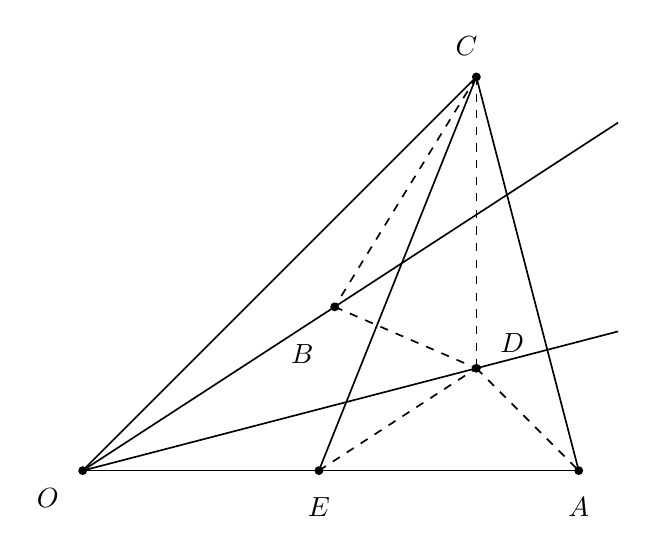
\begin{tikzpicture}[x=1cm,y=1cm,line width=.6pt,font=\normalsize]
% Schematic spatial construction, not a metric projection
\coordinate (O) at (0,0);
\coordinate (E) at (3,0);
\coordinate (A) at (6.3,0);
\coordinate (C) at (5.0000000000,5.0000000000);
\coordinate (D) at (5.0000000000,1.3000000000);
\coordinate (B) at (3.2000000000,2.0800000000);
\coordinate (OBend) at (6.8000000000,4.4200000000);
\coordinate (ODend) at (6.8000000000,1.7680000000);
% base and rays from O
\draw (O)--(E)--(A);
\draw (O)--(C);
\draw (O)--(B)--(OBend);
\draw (O)--(D)--(ODend);
% solid edges from C
\draw (C)--(E);
\draw (C)--(A);
% dashed hidden edges
\draw[dashed] (C)--(B);
\draw[dashed] (C)--(D);
\draw[dashed] (B)--(D);
\draw[dashed] (E)--(D);
\draw[dashed] (D)--(A);
% points
\foreach \p in {O,E,A,C,D,B} {\fill (\p) circle (1.6pt);}
% labels with clearance
\node[anchor=north east,xshift=-5pt,yshift=-3pt] at (O) {$O$};
\node[anchor=north,yshift=-6pt] at (E) {$E$};
\node[anchor=north,yshift=-6pt] at (A) {$A$};
\node[anchor=south east,xshift=4pt,yshift=4pt] at (C) {$C$};
\node[anchor=west,xshift=5pt,yshift=9pt] at (D) {$D$};
\node[anchor=north east,xshift=-4pt,yshift=-10pt] at (B) {$B$};
\end{tikzpicture}
